\subsection{Die Wissenstr�gerschnittstelle}
Bei der Wissenstr�gerschnittstelle handelt es sich um eine Methode zur Datenerfassung, die einen direkten Wissenstransfer zwischen einem Wissenstr�ger und dem Expertensystem erm�glicht. Da die Daten manuell eingegeben und maschinell bearbeitet werden, bezeichnet man die Wissenstr�gerschnittstelle als semi-automatisierte Wissenserfassungsmethode. Im Folgenden werden zwei Anwendungsbeispiele aus unterschiedlichen Bereichen betrachtet und in Bezug auf die wichtigsten Erkenntnisse aus der Entwicklung und dem Einsatz zusammengefasst. \\
Ein Beispiel des Einsatzes der Wissenstr�gerschnittstelle bei einem Elektrotechnikunternehmen wird in \cite{gebus2009} vorgestellt. In der Studie wird ein bereits bestehendes \ac{DSS} untersucht, das die F�hrungskr�fte bei den Entscheidungen von nicht-strukturieren Problemen in der Produktionsabteilung unterst�tzten soll \cite[S.94]{gebus2009}. Das Problem dabei besteht darin, dass das DSS nur eine reine Datensammlung darstellt. Die Produktionsprozesse werden allerdings von Experten gesteuert, die mithilfe des Erfahrungswissens St�rungen in der Produktion beseitigen. Als Folge hat die Unternehmensf�hrung einen begrenzten �berblick �ber die Situation in der Produktionsabteilung. Au�erdem besteht die Gefahr, dass das spezifische Expertenwissen verloren geht falls der Wissenstr�ger das Unternehmen verl�sst.\\
Die Zielsetzung von \cite{gebus2009} ist, das bestehende DSS mit dem Expertenwissen zu erweitern und somit ein wissensbasiertes DSS zu schaffen. Um das erforderliche Wissen aus der Produktion zu sammeln, erweitern Gebus und Leivisk{\"a} das DSS um eine Schnittstelle f�r Anlagenbediener. Die Struktur und Beziehungen vom DSS sind in der Abbildung \ref{dss_gebus} schematisch nachgebildet.
\begin{figure}[H] 
	\centering
	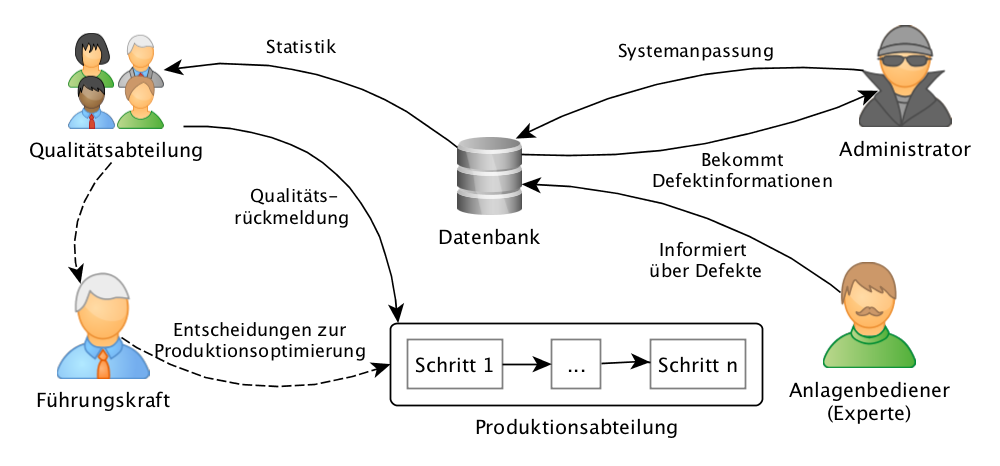
\includegraphics[width=0.9\textwidth]{images/dss_gebus.png}
	\caption{Die Struktur und Beziehungen im \ac{DSS}, \cite[S.98]{gebus2009}}
	\label{dss_gebus}
\end{figure} 